\section{Conclusion}
In this chapter, we have determined three building blocks to capture the specification of coordination patterns: 
\begin{itemize}
	\item a language behavioral interface;
	\item a correspondence rule;
	\item  a coordination rule.
\end{itemize}
Table~\ref{table:framework} summarizes the main characteristics of these elements in the studied approaches. 

\begin{table}[]
	\centering
	\caption{Sumarizes of the studied approaches}
	\label{table:framework}
\begin{tabular}{|c|c|c|c|}
	\hline
	\rowcolor[HTML]{FFFFC7} 
	Approach                                                    & \begin{tabular}[c]{@{}c@{}}Language Behavioral \\ Interface\end{tabular} & \begin{tabular}[c]{@{}c@{}}Correspondence \\ Rule\end{tabular} & \begin{tabular}[c]{@{}c@{}}Coordination \\ Rule\end{tabular} \\ \hline
	\begin{tabular}[c]{@{}c@{}}Ptolemy \\ ModHel'X\end{tabular} & \begin{tabular}[c]{@{}c@{}}methods,\\ generic\end{tabular}               & composite actors                                               & Java                                                         \\ \hline
	MASCOT                                                      & \begin{tabular}[c]{@{}c@{}}methods,\\ wrappers\end{tabular}              & naming convention                                              & C                                                            \\ \hline
	Di Natale                                                   & methods                                                                  & connectors                                                     & C++                                                          \\ \hline
	\rowcolor[HTML]{FFCCC9} 
	BCOoL                                                       & \begin{tabular}[c]{@{}c@{}}Event types\\ domain-specific\end{tabular}    & dedicated language                                             & MOCCML                                                       \\ \hline
\end{tabular}
\end{table}
 
We have identified that a language behavioral interface is a partial representation of the syntax and behavioral semantics of languages for coordination purpose. We have determined that an explicit language behavioral interface has several benefits. For instance, it helps to identify the coordination point thus easing the task to add support to a new language. We have noted that, when the interface is made of events, the specification of the coordination between languages can be done by keeping separately the coordination and the computation concerns. This avoids altering the coordinated language semantic.

We want to highlight that the notion of interface is not presented in model composition approaches. These approaches compose heterogeneous models by relying on a fixed metametamodel. For example, in the Epsilon Comparing Language the metametamodel is always Ecore. However, in the case of behavioral coordination, the models can be built with very different languages, \eg SDL and Matlab in MASCOT. This results in a need of a notion of interface at language level to coordinate both languages.  

We have identified that correspondence rules specify when elements from different languages must be coordinated. From the studied approaches, we have identified two kinds of correspondences. However, we have determined that only the naming convention can be fully automatized without the help of a system designer. We have also noted that none approach relies on a dedicated language (\eg Epsilon Comparison Language) to express the correspondence rule. We have determined that such a language would ease the task of a language integrator to find similarities between models elements.  

Together with a correspondence rule, we have shown that approaches rely on a notion of coordination rule that specifies the behavior of the correspondences. We have noted that all approaches express the coordination in a general purpose language thus limiting verification and validation. We have concluded that none approaches leverage on the work done by Coordination Languages and ADLs in which the coordination rule is explicit and expressed in a formal language.  

\begin{figure}
	\begin{center}
		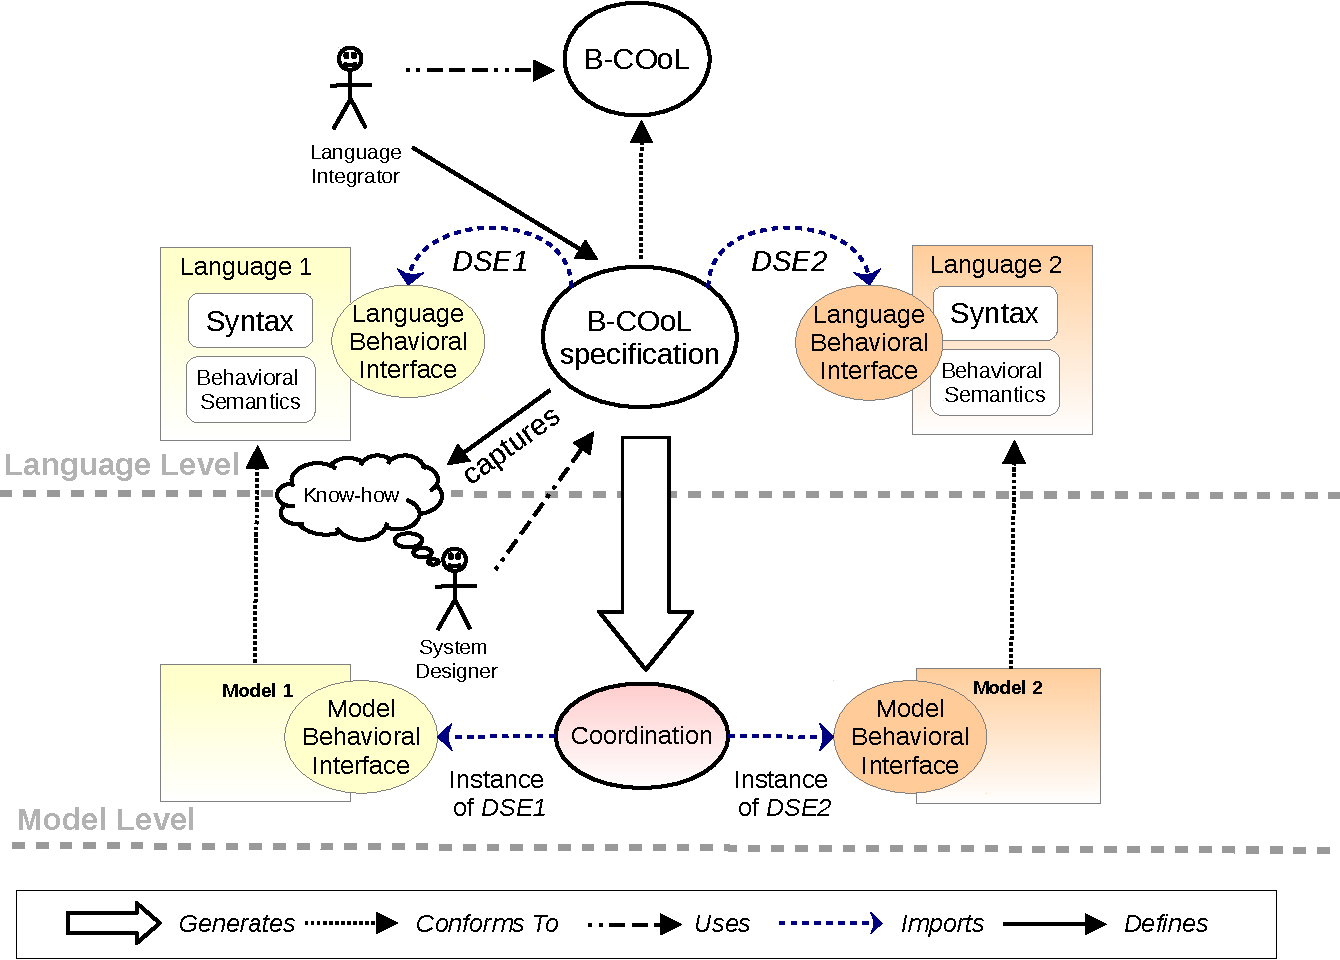
\includegraphics[width=1\textwidth]{framework/figs/bcool}
		\caption{Overview of the Approach}
		\label{fig:bcool}
	\end{center}
\end{figure}

In this thesis, we propose a dedicated language named \bcool to capture coordination patterns between languages. \bcool is an implementation of the framework previously presented (in red in Table~\ref{table:framework}).  
%\begin{enumerate}
%	\item A language behavioral interface made of event types. 
%	\item A correspondence rule expressed in a query language (\eg a matching operator). 
%	\item A coordination rule in a formal language. 
%\end{enumerate}

We base on a language behavioral interface made of event types (\ie \dse\cite{sle13-combemale}) as ``coordination points" to drive the execution of languages. These events are used as handles or control points in two complementary ways: to observe what happens inside the model, and to control what is allowed to happen or not. When required by the coordination, constraints are used to forbid or delay some event occurrences. Forbidding occurrences reduces what can be done by individual models. When several executions are allowed
(nondeterminism), it gives some freedom to individual semantics for making their own choices. All this put together makes the \dse suitable to drive coordinated simulations without being intrusive in the models. 

In \bcool, coordination patterns are captured as constraints at the language level on the \dse (see Figure~\ref{fig:bcool}). To do so, a language integrator defines \emph{Operators} that are composed by a \emph{correspondence matching} and a \emph{coordination rule}. The correspondence matching identifies what elements from the behavioral interfaces (\ie what instances of \dse) must be selected. To do so, we rely on the context in which a \dse is defined to selected instances of such \dse. Then, a coordination rule specifies the, possibly timed, synchronizations and causality relationships between the instances of \dse selected during the matching. To specify the coordination rule, we rely on a CCSL-based language named \moccml~\cite{moccmlbib}. The specification at language level applies between models thus generating a formal model of coordination in \ccsl. This enables a system designer to validate and verify a coordinated system. In the following chapter, we present the implementation of \bcool.
%The design of \bcool is inspired by current structural composition languages (\eg\cite{epsilon,kompose}). These approaches rely on the \emph{matching} and \emph{merging} phases of syntactic model elements. A matching rule specifies what elements from different models are selected. A merging rule specifies how the selected model elements are composed. In these approaches the specification is at the language level, but the application is between models. Similarly, a \bcool operator relies on a \emph{correspondence matching} and a \emph{coordination rule}. The correspondence matching identifies what elements from the behavioral interfaces (\ie what instances of \dse) must be selected. The merging phase is replaced by a coordination rule. While in the structural case the merging operates on the syntax, the coordination rule operates on elements of the semantics (\ie instances of \dse). Thus, coordination rules specify the, possibly timed, synchronizations and causality relationships between the instances of \dse selected during the matching.
